\chapter{Opis i wyniki przeprowadzonych testów}

\section{Przebieg procesu testowania}
Część praktyczna pracy polegała na implementacji programu do klasteryzacji dokumentów tekstowych oraz przeprowadzeniu testów weryfikujących skuteczność opracowanego rozwiązania. Opracowany system na wejściu otrzymuje listę dokumentów tekstowych w postaci pliku ".csv", a w rezultacie tworzy nowy plik ".csv" z listą dokumentów tekstowych oraz przypisanymi do nich etykietami klastrów. Przygotowanie takiego projektu składało się z kilku etapów:
\begin{itemize}
    \item znalezienie dużego zbioru dokumentów tekstowych potrzebnego do przeprowadzenia testów weryfikujących skuteczność systemu,
    \item przetworzenie dokumentów tekstowych na format akceptowalny przez procedury wykorzystane do implementacji klasteryzacji,
    \item implementacja systemu do wstępnego przetwarzania i klasteryzacji dokumentów tekstowych,
    \item przeprowadzenie testów weryfikujących skuteczność wybranej metody klasteryzacji.
\end{itemize}
\newpage

Celem eksperymentu jest znalezienie jak najbardziej podobnych do siebie dokumentów, korzystając tylko z metod przetwarzania dokumentów tekstowych oraz klasteryzacji. W pracy zostały wykorzystane takie metody jak, "stemming", "tf-idf".

Problem polega na tym, że klasteryzacja, inaczej zwana klasyfikacją nienadzorowaną, zwraca podzielone dokumenty na grupy w różny sposób. Interpretacja wygenerowanych klastrów wymaga zastosowania kilku metod w celu weryfikacji czy dany wynik jest poprawny bądź nie. Dokumenty tekstowe znajdujące się w zbiorze testowym posiadają etykiety opisujące ich przynależność do predefiniowanych klas. Zatem weryfikacja skuteczności klasteryzacji będzie polegała na porównaniu dla każdego dokumentu jego klasy referencyjnej z klasą przypisaną mu przez algorytm klasteryzacji.

\section{Wykorzystane dane do przeprowadzenia eksperymentów}
Do przeprowadzenia eksperymentów został wykorzystany zbiór danych znalezionych na jednej ze stron internetowych \cite{datasetclass} o nazwie roboczej \texttt{"ag\_news\_csv"}. Dokumenty tekstowe zawarte w tym zbiorze są podzielone na 4 grupy.

\begin{table}[h!]
    \centering
    \caption{Klasy z danego zbioru danych}
    \label{datasetclasses}
    \begin{tabular}{|l|l|l|l|l|}
    \hline
    Numer klasy & 1     & 2      & 3        & 4        \\ \hline
    Nazwa klasy & World & Sports & Business & Sci/Tech \\ \hline
    \end{tabular}
\end{table}

Zbiór danych zawiera w sobie dwa pliki \texttt{"test.csv"} oraz \texttt{"train.csv"}. Ilość dokumentów dla obu plików jest różna i prezentuje się w taki sposób:

\begin{table}[h!]
    \centering
    \caption{Ilość dokumentów tekstowych w poszczególnych klasach i zbiorach danych}
    \label{quantityOfDocs}
    \begin{tabular}{|l|l|l|}
    \hline
    Numer klasy & test.csv & train.csv \\ \hline
    1           & 1900     & 30000     \\ \hline
    2           & 1900     & 30000     \\ \hline
    3           & 1900     & 30000     \\ \hline
    4           & 1900     & 30000     \\ \hline
    \end{tabular}
\end{table}
Struktura w pliku z danymi źródłowymi jest taka, że każda nowa linia to osobny dokument tekstowy. Informacje rozdzielone są separatorem przecinka. W pliku są trzy informacje, takie jak numer klasy oryginalnej, nazwa artykułu oraz treść artykułu. 

Powodem dla którego został wybrany ten zbiór danych, jest fakt, że zbiór ten nie posiada dużo klas, dzięki czemu stopień trudności klasteryzacji jest mniejszy. Wydobycie cech z dokumentów tekstowych w podanym zbiorze, możliwe jest dzięki odpowiedniej długości słów w nich zawartych.

W wypadku, gdy dokument tekstowy będzie zbyt krótki, po całym procesie przetwarzania może nie mieć ani jednej cechy opisującej ten dokument. Cechami w tym przypadku są częstości występowania słów kluczowych, których lista ustalana jest w wyniku przetwarzania wstępnego wszystkich tekstów.


Podczas analizowania treści tych dokumentów, napotkałem na wiele różnych elementów, które nie wnoszą nic do ich istotności. Są to m.in. adresy URL, akronimy, czy elementy znaczników HTML, ponieważ dokumenty tekstowe w podanym zbiorze pochodzą ze stron internetowych, dlatego w kilku przypadkach parsowanie i kasowanie HTML nie zadziałało poprawnie. Takie elementy mogą zakłócić działanie algorytmu. Bardzo ważny jest moment przetwarzania dokumentów tekstowych, tak by zostały w nim tylko istotne słowa.
\newpage

\section{Cele szczegółowe}
    \subsection{Parsowanie HTML}
    Niektóre dokumenty z podanego zbioru posiadają w sobie różnego rodzaju znaczniki HTML czy nawet adresy URL, które są zbędnymi słowami jeśli chodzi o klasteryzację. W tym celu została napisana metoda, która przyjmuje treść dokumentu tekstowego jako parametr i zwraca ten sam dokument bez znaczników i znaków specjalnych takich jak "\&lt;". Metody te korzystają z bibliotek "html" oraz "re" dostarczonych przez język Python.
    
    \lstinputlisting[label={lst:3.4},caption={Metody do kasowania znaczników HTML oraz adresów URL}, language=python, showstringspaces=false, breaklines=true]{Algorytmy/Rozdzial3/parsehtml.py}   
    
    Obie metody można wykorzystać w funkcji "PrepareDocument", która została zaprezentowana w rozdziale \ref{lst:3.2}.
    
    Metoda "RemoveHTMLTags" przyjmuje jako parametr dokument tekstowy. W pierwszej kolejności korzysta z metody "html.unescape", która zamienia wszystkie znaki specjalne (np. \&gt;, \&\#62;), na ich odpowiedniki w formacie Unicode.  Następnie poprzez użycie wyrażeń regularnych usuwa znaczniki HTML, bez kasowania ich zawartości. Metoda "RemoveUrl" również przyjmuje dokument tekstowy jako parametr. Korzystając z wyrażenia regularnego na danym tekście, wszystkie znalezione wzorce są zamieniane na pusty tekst.
    
    
    \subsection{Schemat działania algorytmu} \label{sec:alg}
    \begin{figure}[h!]
        \centering
        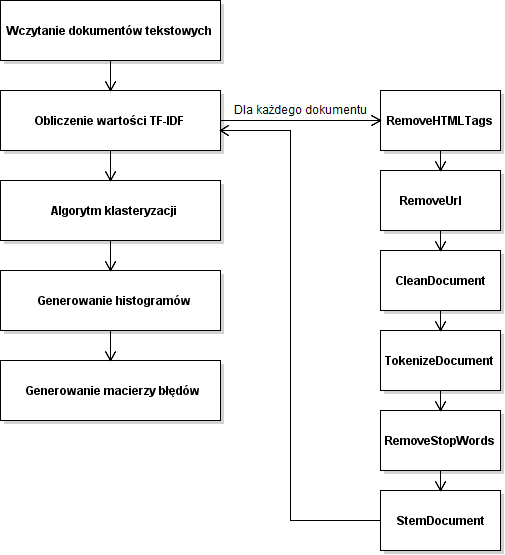
\includegraphics[scale=0.6]{Rysunki/Rozdzial3/diagram.png}
        \caption{Diagram przedstawiający etapy działania programu do klasteryzacji dokumentów tekstowych}
        \label{fig:diagram}
    \end{figure}
    Na samym początku należy skonfigurować algorytm, tak by działał z odpowiednimi danymi. W przypadku algorytmu k-means należy określić, na ile klas chcemy podzielić dane. Należy również określić ścieżkę dostępu do pliku \texttt{".csv"} ze zbiorem danych, oraz nazwami klas. Kolejnym etapem jest pobranie wszystkich dokumentów tekstowych do listy.
    \newpage
    \lstinputlisting[label={lst:3.1},caption={Pobieranie dokumentów tekstowych z pliku .csv}, language=python, showstringspaces=false, breaklines=true]{Algorytmy/Rozdzial3/getFile.py}
    
    Dalej, wszystkie dokumenty są przygotowywane zgodnie z wymaganiami. Przygotowanie dokumentu tekstowego dzieli się na 4 etapy:
    \begin{enumerate}
        \item czyszczenie (patrz \ref{sec:czyszczenie}),
        \item tokenizacja (patrz \ref{sec:tokenizacja}),
        \item usuwanie słów zawartych w stop liście ,
        \item normalizacja, czyli stemming (patrz \ref{sec:normalizacja}).
    \end{enumerate}
    
    \lstinputlisting[label={lst:3.2},caption={Implementacja metod odpowiedzialnych za przygotowanie dokumentów tekstowych}, language=python, showstringspaces=false, breaklines=true]{Algorytmy/Rozdzial3/prepareDoc.py}
    
    Parametr "tokenizer" wymusza wykorzystanie naszej metody do celów tokenizacji, który dodatkowo ma zaimplementowane inne elementy przygotowania dokumentu tekstowego. Na samym końcu uruchomiamy algorytm klasteryzacji.
    \lstinputlisting[label={lst:3.3},caption={Uruchomienie algorytmu k-Means}, language=python, showstringspaces=false, breaklines=true]{Algorytmy/Rozdzial3/kmeans.py}
    
    Algorytm k-means \ref{sec:kmeans} w bibliotece Scikit-learn zwraca listę przypisanych klas do dokumentów tekstowych w takiej samej kolejności, w jakiej otrzymał je na wejściu.
    
    \subsection{Weryfikacja poprawności rezultatów}
    Algorytm klasteryzacji ma jedną istotną wadę: numery klastrów, które zostały zwrócone, nie muszą odzwierciedlać faktycznych klas dokumentów tekstowych. Dlatego też ważnym elementem jest poprawna weryfikacja jakości wyników. W pracy opisane zostaną dwie metody weryfikacji zwróconych klas. 
    
    Dokumenty tekstowe ze zbioru danych posiadają już przypisaną klasę do każdego dokumentu. Ta wiedza jest istotna podczas generowania macierzy pomyłek \ref{sec:confusion}. Weryfikacja dokładności klasyfikacji dokumentów za pomocą klasteryzacji odbywa się kilkuetapowo:
    
    \begin{itemize}
        \item wygenerowanie macierzy pomyłek, dla predykowanych klas wygenerowanych za pomocą algorytmu klasteryzacji,
        \item wygenerowanie histogramu z rozkładem klas w poszczególnych klastrach,
        \item zmapowanie na nowo predykowanych klas, korzystając z informacji z histogramu, oraz wygenerowanie macierzy pomyłek,
        \item zmapowanie predykowanych klas na wszystkie sposoby prezentacji, wygenerowanie dla każdej kombinacji macierzy pomyłek, oraz policzenie trafności przypisanych klas.
    \end{itemize}
\newpage
\section{Wyniki testów}
    Wykorzystując przedstawione w poprzednim punkcie kroki, istnieje możliwość zbadania wyników klasteryzacji na danym zbiorze danych \texttt{"ag\_news\_csv"}. 
    
    Na początku zostały przedstawione wyniki z pierwszego uruchomienia algorytmu na pliku "test.csv", który zawiera po 1900 dokumentów tekstowych z każdego klastra.
    
    Uruchomienie programu na zbiorze testowym, wyświetli 4 wykresy w osobnych oknach. Wykresy zostały przedstawione oraz omówione na rysunkach \ref{fig:r11}, \ref{fig:r12}, \ref{fig:r13} i \ref{fig:r15}.
    
    \begin{figure}[h!]
        \centering
        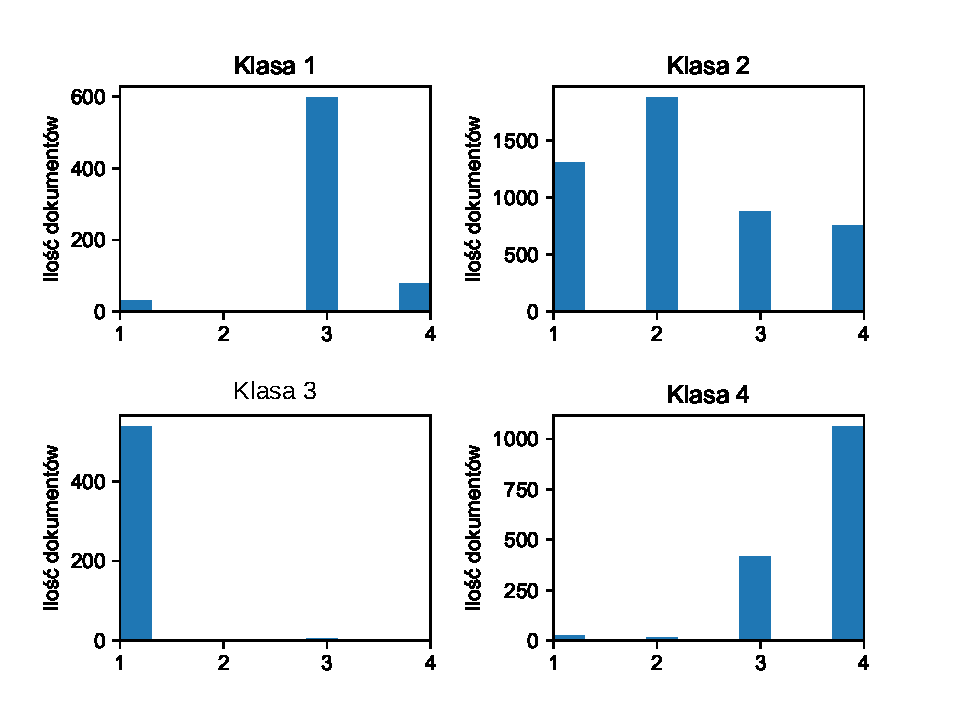
\includegraphics[scale=0.8]{Rysunki/Rozdzial3/edited_run11.pdf}
        \caption{Uruchomienie 1: Histogram}
        \label{fig:r11}
    \end{figure}
    
    Wygenerowane na powyższym rysunku \ref{fig:r11} histogramy, odzwierciedlają ilość przypisanych klas przez algorytm klasteryzacji do dokumentów tekstowych należących do predefiniowanej klasy.
    
    Poniższy rysunek \ref{fig:r12} przedstawia macierz błędu. Został on wygenerowany na podstawie etykiet rzeczywistych oraz predykowanych zwróconych przez algorytm klasteryzacji.
    
    \begin{figure}[h!]
        \centering
        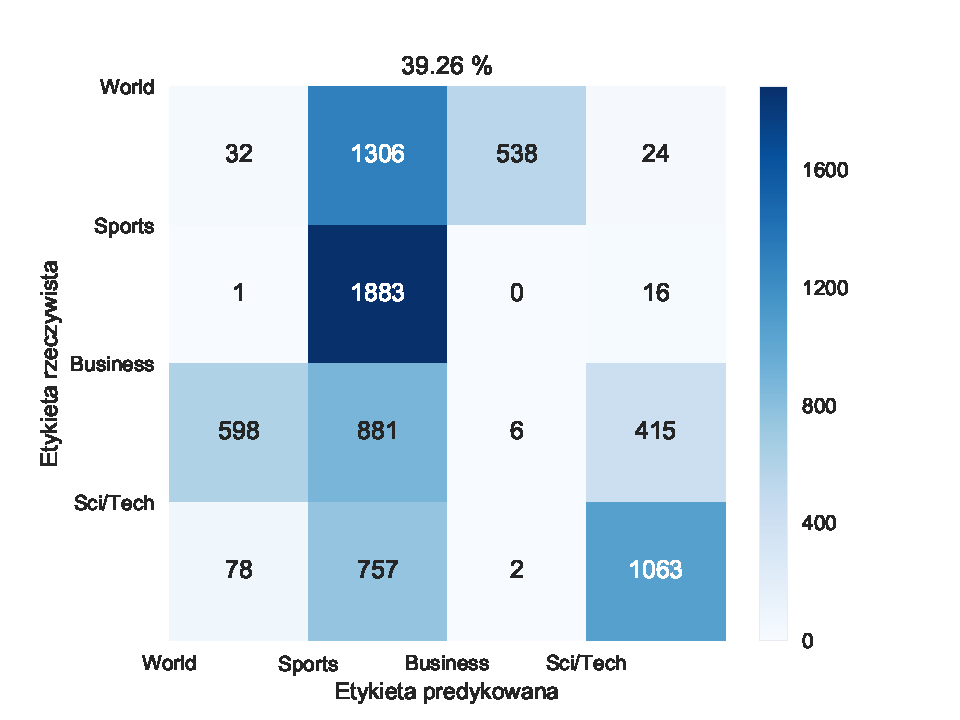
\includegraphics[scale=0.6]{Rysunki/Rozdzial3/run12.pdf}
        \caption{Uruchomienie 1: Macierz błędu dla danych zwróconych z algorytmu}
        \label{fig:r12}
    \end{figure}
    
    \newpage
    Nazwą macierzy jest policzona metryka trafności (ang. accuracy) wyników. Idealne uruchomienie posiadałoby trafność na poziomie 100 \%, a macierz miałaby wszystkie dokumenty tekstowe znalezione po przekątnej. Na tym etapie wynik poprawności algorytmu klasteryzacji dla tego zbioru danych to 39.26 \%. 
    
    Można jednak spróbować zrobić nowe mapowanie klas odkrytych przez algorytm, dzięki wcześniej wygenerowanemu histogramowi \ref{fig:r11}. Zakładając, że dla dokumentów z klasy "1" algorytm przypisał nowe etykiety, to uznać można, że klasa predykowana "3" jest naszą oryginalną "1". Tak samo postępujemy z kolejnymi histogramami. Dzięki temu można przyjąć nowe mapowanie klas. 
    
    \begin{table}[h!]
        \centering
        \caption{Uruchomienie 1: Nowe mapowanie klas predykowanych}
        \label{newMapPred}
        \begin{tabular}{|l|l|}
        \hline
        Jaka klasa & Predykowana klasa \\ \hline
        1          & 3                 \\ \hline
        2          & 2                 \\ \hline
        3          & 1                 \\ \hline
        4          & 4                 \\ \hline
        \end{tabular}
    \end{table}
    
    W przedstawionym przypadku należy zamienić wszystkie "3" na "1" oraz "1" na "3". Takie mapowanie utworzy nową listę etykiet, a macierz błędu wyglądać będzie następująco:
    \newpage
    \begin{figure}[h!]
        \centering
        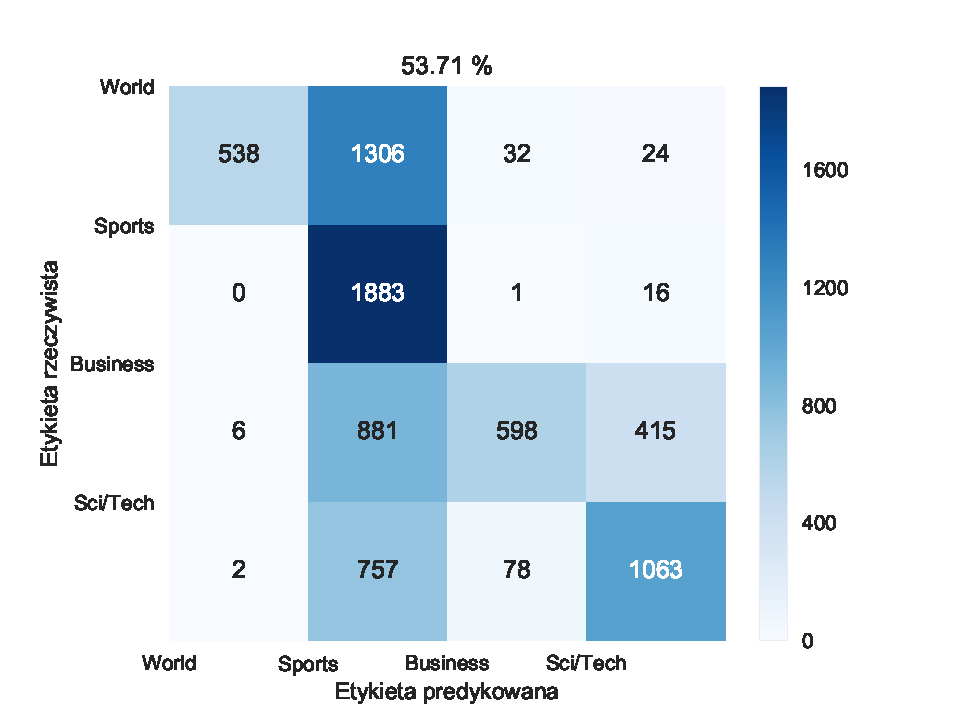
\includegraphics[scale=0.57]{Rysunki/Rozdzial3/run13.pdf}
        \caption{Uruchomienie 1: Macierz błędu dla danych po zmapowaniu etykiet z histogramów}
        \label{fig:r13}
    \end{figure}    
    
    Takie mapowanie klas, zwiększyło trafność, aż do 53.71 \%. 
    
    Na koniec należy skorzystać jeszcze z jednej opcji weryfikacji poprawności danych. Zamiana predykowanych klas w różnych kombinacjach przedstawiona została w \ref{sec:zamianaKlas}. Mapowanie w ten sposób klas pokazało, że takie kombinacje nie są na tyle dobre, aby uznać je za poprawne. Dzieje się tak chociażby ze względu na to, że mapowanie z histogramu dało lepszy rezultat.
    
    \begin{figure}[h!]
        \centering
        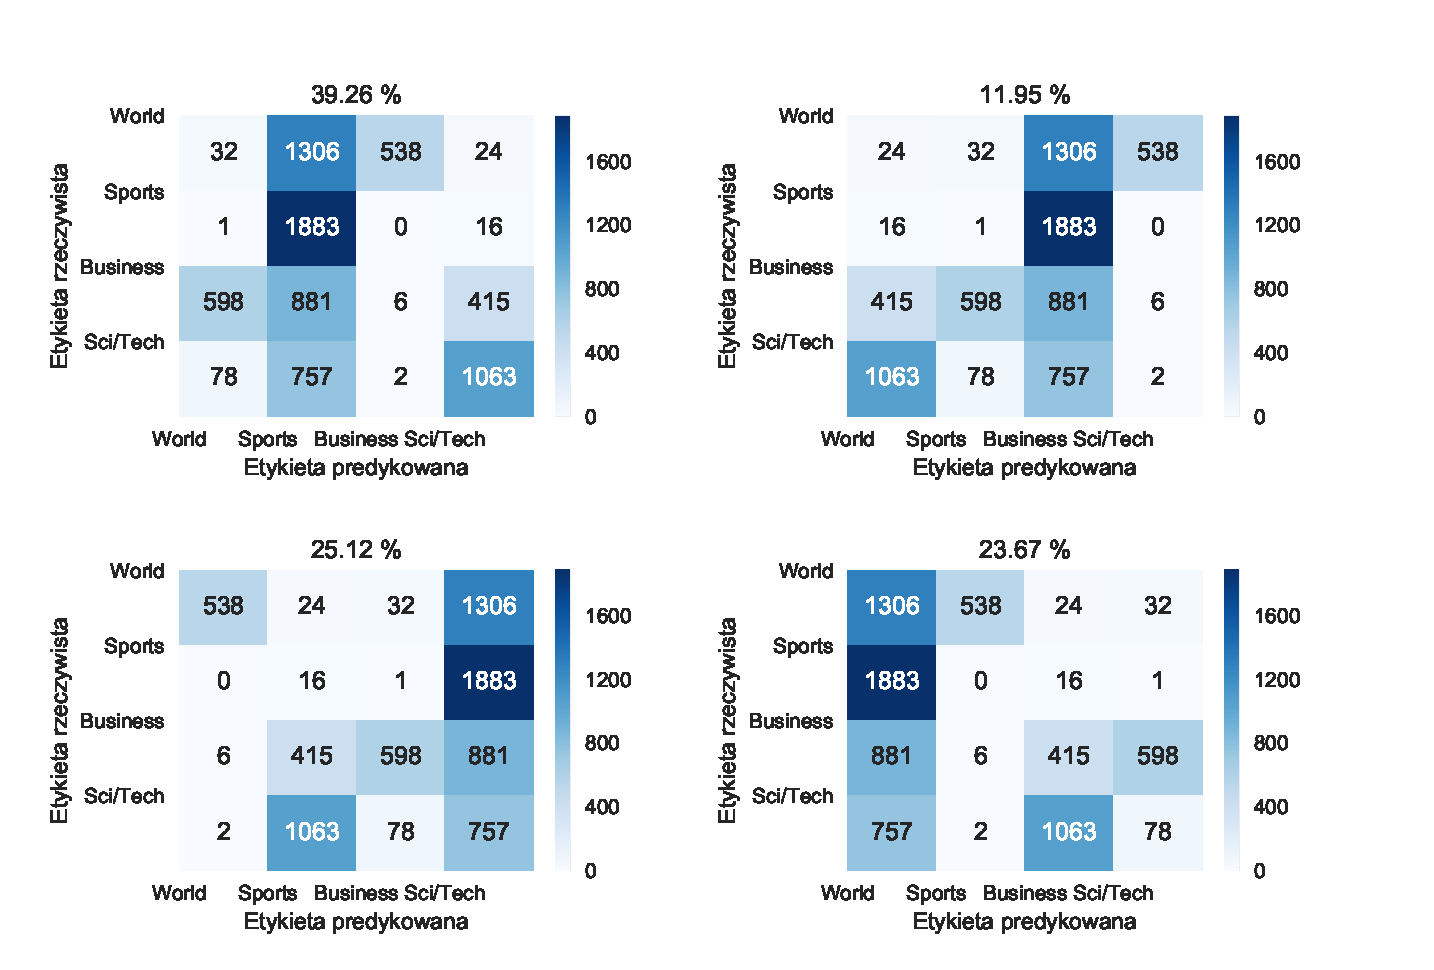
\includegraphics[scale=0.57]{Rysunki/Rozdzial3/run15.pdf}
        \caption{Uruchomienie 1: Macierze błędów po dokonaniu zamiany klas}
        \label{fig:r15}
    \end{figure}
    Dla pierwszego uruchomienia, przypisanie klas z \ref{newMapPred} jest najlepszym mapowaniem.
    Na tych danych algorytm klasteryzacji został uruchomiony 5 razy, na trzech różnych progach ilości przeprowadzonych iteracji: 10, 100 i 400. Tak prezentują się wyniki poszczególnych uruchomień.
    \begin{table}[h!]
        \centering
        \caption{Najlepsze wyniki dla 5 uruchomień na zbiorze danych "test"}
        \label{bestAccTest}
        \begin{tabular}{|c|c|c|c|}
        \hline
        Lp. & \begin{tabular}[c]{@{}c@{}}Najlepsza trafność \\ dla 10 iteracji\end{tabular} & \begin{tabular}[c]{@{}c@{}}Najlepsza trafność \\ dla 100 iteracji\end{tabular} & \begin{tabular}[c]{@{}c@{}}Najlepsza trafność \\ dla 400 iteracji\end{tabular} \\ \hline
    1 & 53.38 \% - Zamiana klas & 50.63 \% - Histogram & 53.71 \% - Histogram \\ \hline
    2 & 62.38 \% - Zamiana klas & 58.92 \% - Histogram & 53.62 \% - Histogram \\ \hline
    3 & 33.33 \% - Zamiana klas & 52.86 \% - Histogram & 53.34 \% - Zamiana klas \\ \hline
    4 & 64.07 \% - Zamiana klas & 52.76 \% - Zamiana klas & 53.33 \% - Histogram \\ \hline
    5 & 37.75 \% - Zamiana klas & 59.68 \% - Histogram & 59.95 \% - Histogram \\ \hline
        \end{tabular}
    \end{table}
    
    Średnie procentowe wyniki trafności na wyznaczonych progach są do siebie dość podobne. Dla 10 iteracji średnia trafności jest mniejsza o 4 punkty procentowe. Można również zauważyć pewną zależność: czym mniej iteracji tym lepsza trafność prezentowana była w sposobie weryfikacji zamiany klas. Natomiast w liczbie iteracji od 100 do 400, sposób mapowania zwykle opierał się na bazie histogramu.
    
    Zastosowanie sposobów weryfikacji na zbiorze danych zawierających 30000 dokumentów tekstowych dało gorsze wyniki przy uruchomieniu na 10 iteracjach.
    \begin{table}[h!]
        \centering
        \caption{Najlepsze wyniki dla 3 uruchomień na zbiorze danych "train"}
        \label{bestAccTrain}
        \begin{tabular}{|c|c|c|c|}
        \hline
        Lp. & \begin{tabular}[c]{@{}c@{}}Najlepsza trafność \\ dla 10 iteracji\end{tabular} & \begin{tabular}[c]{@{}c@{}}Najlepsza trafność \\ dla 100 iteracji\end{tabular} & \begin{tabular}[c]{@{}c@{}}Najlepsza trafność \\ dla 400 iteracji\end{tabular} \\ \hline
        1 & 38.66 \% - Zamiana klas & 51.7 \% - Histogram & 34.53 \% - Zamiana klas \\ \hline
        2 & 33.45 \% - Zamiana klas & 34.54 \% - Zamiana klas & 51.77 \% - Zamiana klas \\ \hline
        3 & 43.72 \% - Zamiana klas & 51.8 \% - Zamiana klas & 51.66 \% - Zamiana klas \\ \hline
        \end{tabular}
    \end{table}